\begin{figure}[!h]
    \centering
    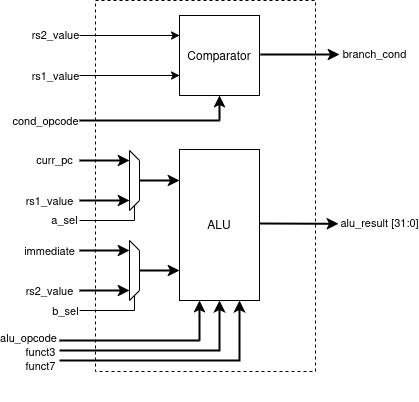
\includegraphics[scale=0.4]{IE_BD.png}
    \caption{A block diagram for the execution stage}
    \label{fig:IE_BD}
\end{figure}
\section{Executing Arithmetic and Logic operations}
With the previous information extrapolated from the instruction, there is now the need to elaborate the incoming values stored in their relative registers, by performing the needed operation type.
The Instruction Execute stage, implemented in the simplest way possible can be described in VHDL with two main blocks:
\begin{itemize}
\item \textbf{Comparator}: takes two 32-bit inputs and returns a boolean value indicating wether or not the comparison between the two inputs follow a decided criteria. This block is dedicated to the branch-type instructions, that may end in an instruction jump.
\item \textbf{Arithmetic-Logic Unit}: performs all other arithmetic and logic operations, while also handling shifts. When coding this block it has to be taken into account that both signed and unsigned operations have to be performed. For this reason the inputs of each multiplexer will be casted as unsigned at first (to match for the immediate values already being unsigned) and then casted correctly afterwards. 
\end{itemize}
Starting from the ALU, being the most complex of the two, the necessary steps to take before the description is to understand what type of operation has to be done for each core instruction. As said earlier, some of them can be recognized for both the presence of \emph{funct3} (bit 14 to 12) and \emph{funct7}, in case of R-type onstructions, or just \emph{funct3}. As specified in the base RV32I manual, the univocal codes for the basic core instructions are listed below in table \ref{table:core_instr_funct3}, from which it is easy to notice that the actual purpose of \emph{funct7} is to switch between addition and substraction, since they are encoded as "000", or between logic and arithmetic right shift (in the table SRA and SRL). A simple solution could be editing the behavior of the decoder to have it look at the sixth bit of \emph{funct7} and have all subtractions encoded as "010", as it would happen for SLT, and similarly for SRL and SRA. This solution would remove the necessity for \emph{funct7} and shrink the necessary opcode for the ALU to 3 bits. However, that portion of the instruction, seemingly unnecessary for RV32I, comes useful when implementing floating-point instructions and multiplications, hence the most flexible solution, however complex, is to make the decoder return \emph{funct7} and have the ALU taking it into account when switch between operations.
With this in mind now the decoder can be edited to return \emph{funct7} when treating opcodes mapped as OP, and some instances of OP-IMM when treating shifts.With this being said, it is decided that the ALU can switch operation by taking into account, in order of importance: the instruction class, \emph{funct3} and, to maintain flexibility for future modifications, \emph{funct7}.

\begin{table}[h!]
    \begin{center}
        \begin{tabular}{|c|c|c|c|c|}
            \hline
            class & funct7 & funct3 & instruction & operation \\
            \hline
            \multirow{10}{*}{OP} & 0000000 & 000 & ADD & addition\\
            & 0100000 & 000 & SUB & subtraction\\
            & 0000000 & 001 & SLL & left logic shift\\
            & 0000000 & 010 & SLT & set if less than\\
            & 0000000 & 011 & SLTU & set if less than unsigned\\
            & 0000000 & 100 & XOR & bit-wise EXOR\\
            & 0000000 & 101 & SRL & right logic shift\\
            & 0100000 & 101 & SRA & right arithmetic shift\\
            & 0000000 & 110 & OR & bit-wise OR\\
            & 0000000 & 111 & AND & bit-wise AND\\
            \hline
            \multirow{9}{*}{OP-IMM} & - & 000 & ADDI & addition\\
            & 0000000 & 001 & SLLI & left logic shift\\
            & - & 010 & SLTI & set if less than\\
            & - & 011 & SLTIU & set if less than unsigned\\
            & - & 100 & XORI & bit-wise EXOR\\
            & 0000000 & 101 & SRLI & right logic shift\\
            & 0100000 & 101 & SRAI & right arithmetic shift\\
            & - & 110 & ORI & bit-wise OR\\
            & - & 111 & ANDI & bit-wise AND\\
            \hline
            \multirow{3}{*}{STORE} & - & 000 & SB & addition\\
            & - & 001 & SH & addition\\
            & - & 010 & SW & addition\\
            \hline
            \multirow{5}{*}{LOAD} & - & 000 & LB & addition\\
            & - & 001 & LH & additionn\\
            & - & 010 & LW & addition\\
            & - & 100 & LBU & unsigned addition\\
            & - & 101 & LHU & unsigned addition\\
            \hline
            JALR & - & 000 & JALR & addition\\
            \hline
            JAL & - & - & JAL & addition\\
            \hline
            LUI & - & - & LUI (pseudo instruction LI) & addition with x0\\
            \hline
            AUIPC & - & - & AUIPC & addition\\
            \hline
        \end{tabular}
        \caption{RV32I core instruction, excluding B-type instructions, which will be addressed later}
        \label{table:core_instr_funct3}
    \end{center}
\end{table}

If the ALU can be defined as a big case statement as for the decoder, Table \ref{table:core_instr_funct3} may help to simplify the code, in fact some observations can be already made fro basic optimizations:
\begin{enumerate}
\item Many instructions expect the ALU to perform an addition, thus if the architecture of the block is written as a case statement, \emph{the addition can be performed if no other case applies}.
\item All load and store operations require \emph{funct3} to be used later during WriteBack stage because they may operate with less than 32 bits, thus it can be useful to \emph{pass it down to the latest stages of the datapath}.
\item Shift operations using immediates are encoded as I-type but they just need five bits indicated as \emph{shamt} (shift amount), for shifting more than 32-bits would not make any sense. While this does not affect SLLI and SRLI, the presence of \emph{funct7} rises a problem with SRAI. \emph{Shifts with immediates need to filter part of the second operand}.
\end{enumerate}
The code for the ALU will thus check the operation class, funct3 and funct7 in the latter sequence:
\begin{minted}[fontsize=\footnotesize]{vhdl}
when "00001" => --OP and OP-IMM
    case funct3 is
        when "001" => -- SLL,SLLI
            -- ...
        when "010" => -- SLT,SLTI
            -- ...
        when "011" => -- SLTU,SLTIU
            -- ...
        when "100" => -- XOR, XORI
            -- ...
        when "101" => -- right shifts
            alu_pre_result <= 
                -- ...
            when funct7(5) = '1' else
                -- ...
        when "110" => -- OR,ORI
            -- ...
        when "111" => -- AND, ANDI
            -- ...
        when others =>
            alu_pre_result <= 
                -- ...
            when funct7(5) = '1' else
                -- ...
        end case;
        -- etc...
\end{minted}

\section{Managing Branch instructions}
\let\cleardoublepage\clearpage